\chapter{Results}\label{chapter:results}

The findings of the research is presented in this chapter in the form of the annotation statistics and the retrieval effectiveness of the annotations. The annotation statistics covers the time taken to annotate each annotation methodology, and details about the number of annotations collected. The retrieval effectiveness section provides a breakdown of the performance of both the manually and automatically collected annotations.

\section{Annotation Statistics}

In total, five annotators managed to annotate a total of 10,982 images across all annotation methodologies. These annotators consist of students and staff from an information retrieval group at QUT. Figure \ref{fig:annotator-breakdown} illustrates the number of annotations completed by each annotator. Two annotators account for the majority of the annotations, while three others provide an additional 904. The exact number of each annotation type, the total time it took to annotate each annotation type and the average time it took to annotate is displayed in Table \ref{table:annotation-stats}.

\begin{table}[b]
    \centering
    \begin{tabular}{ | l | l | l | l | p{5cm} |}
    \hline
    Name & Count & Average Time & Total Time \\ \hline
    Text & 3172 & 1 minute & 2 days, 23 hours \\ \hline
    Tag & 2897 & 31 seconds & 23 hours, 40 minutes \\ \hline
    Query & 3616 & 16 seconds & 15 hours, 10 minutes \\ \hline
    Assessment & 1327 & 58 seconds & 21 hours, 36 minutes \\ \hline
    \end{tabular}
    \caption{Annotation statistics obtained by taking the average across all five annotators}
    \label{table:annotation-stats}
\end{table}

\begin{figure}[h]
    \centering
    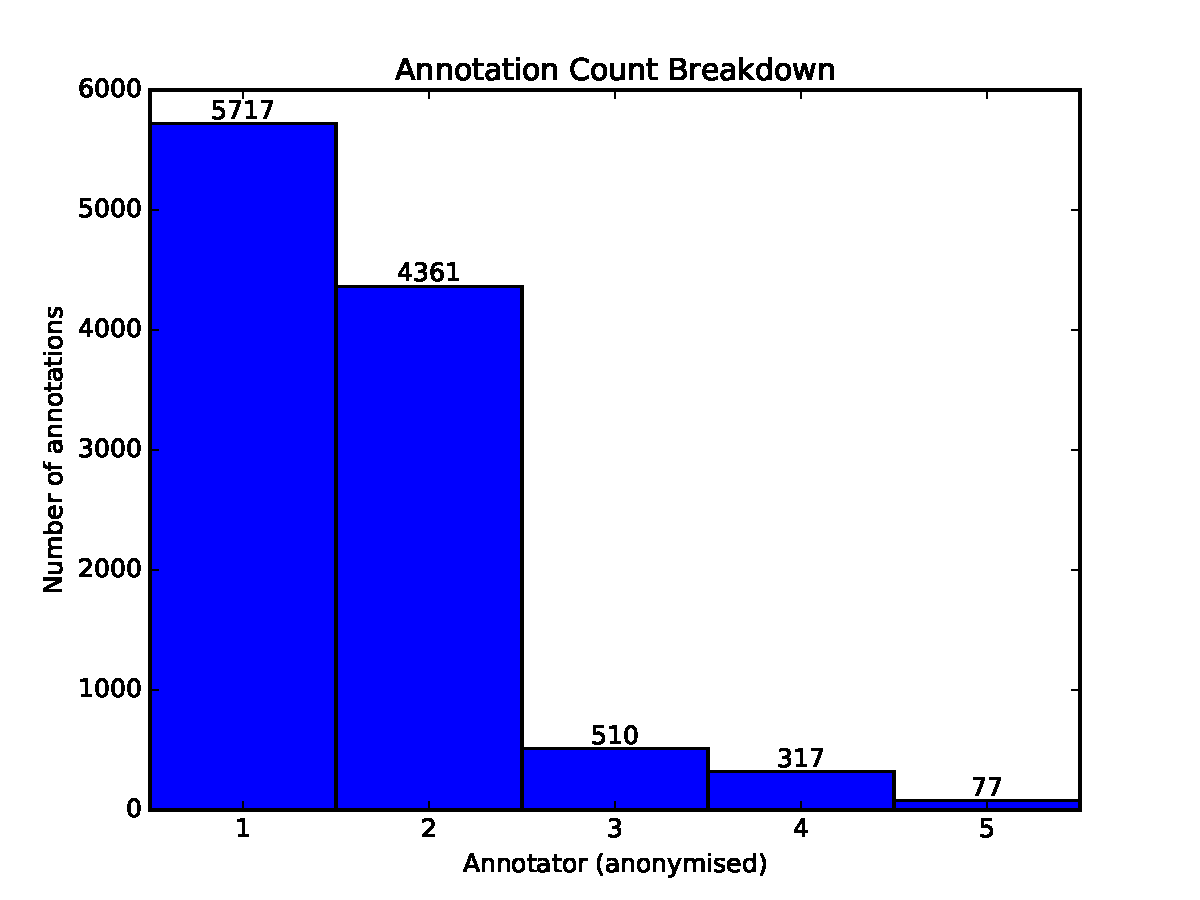
\includegraphics[width=0.8\textwidth]{graphs/annotator-breakdown}
    \caption{Total number of annotations by annotator}
    \label{fig:annotator-breakdown}
\end{figure}

A statistical analysis of the collected annotations reveals that they are appropriate for a typical textual corpus. Figures \ref{fig:idf-scores} and \ref{fig:tf-scores} are what one would expect to see in a Zipfian distribution~\cite{tullo2003modelling}; that is the frequency of each concept is inversely proportional to it's rank in the frequency distribution (the most commonly used concept appears twice as many times as the second most frequent concept and three times as often as the third most frequent concept). The notion of concepts are different to terms since a concept can contain more than one word (this is possible through tags, where a tag can contain multiple words such as `shopping mall' and `street sign').

\begin{figure}[b]
    \centering
    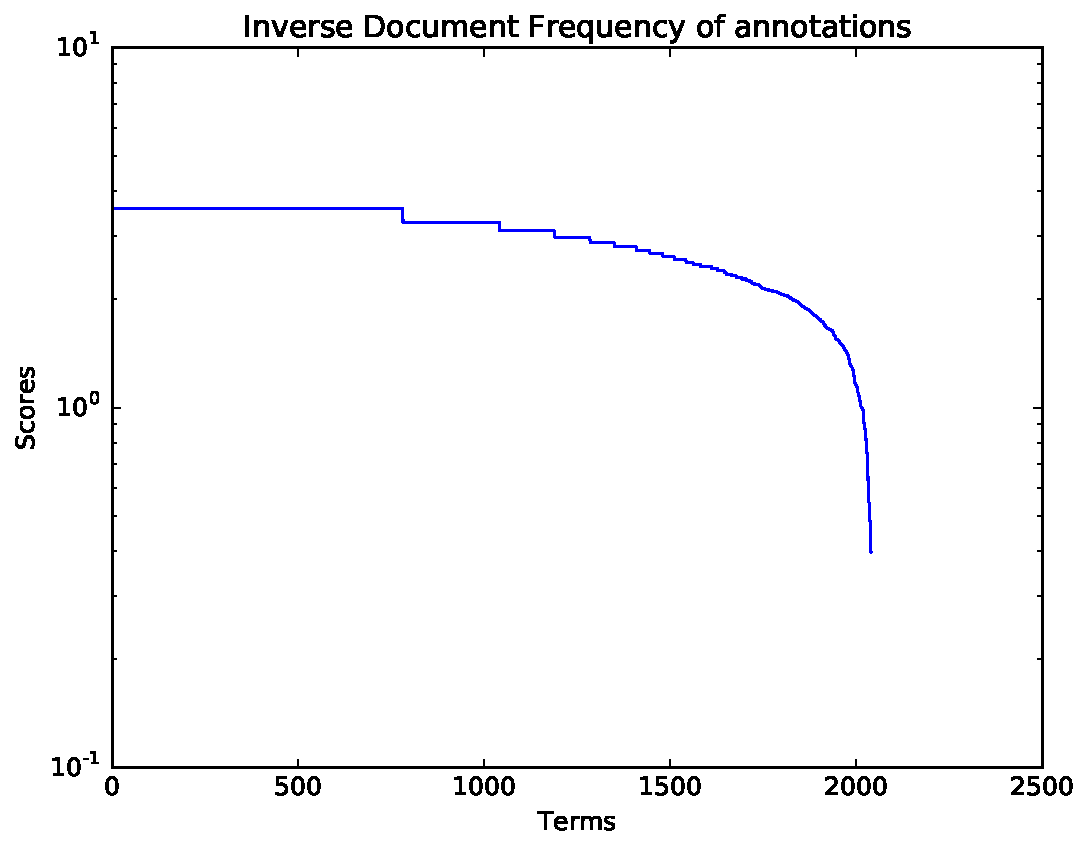
\includegraphics[width=0.7\textwidth]{graphs/idf-scores}
    \caption{IDF scores for concepts in the annotations}
    \label{fig:idf-scores}
\end{figure}

\begin{figure}[b]
    \centering
    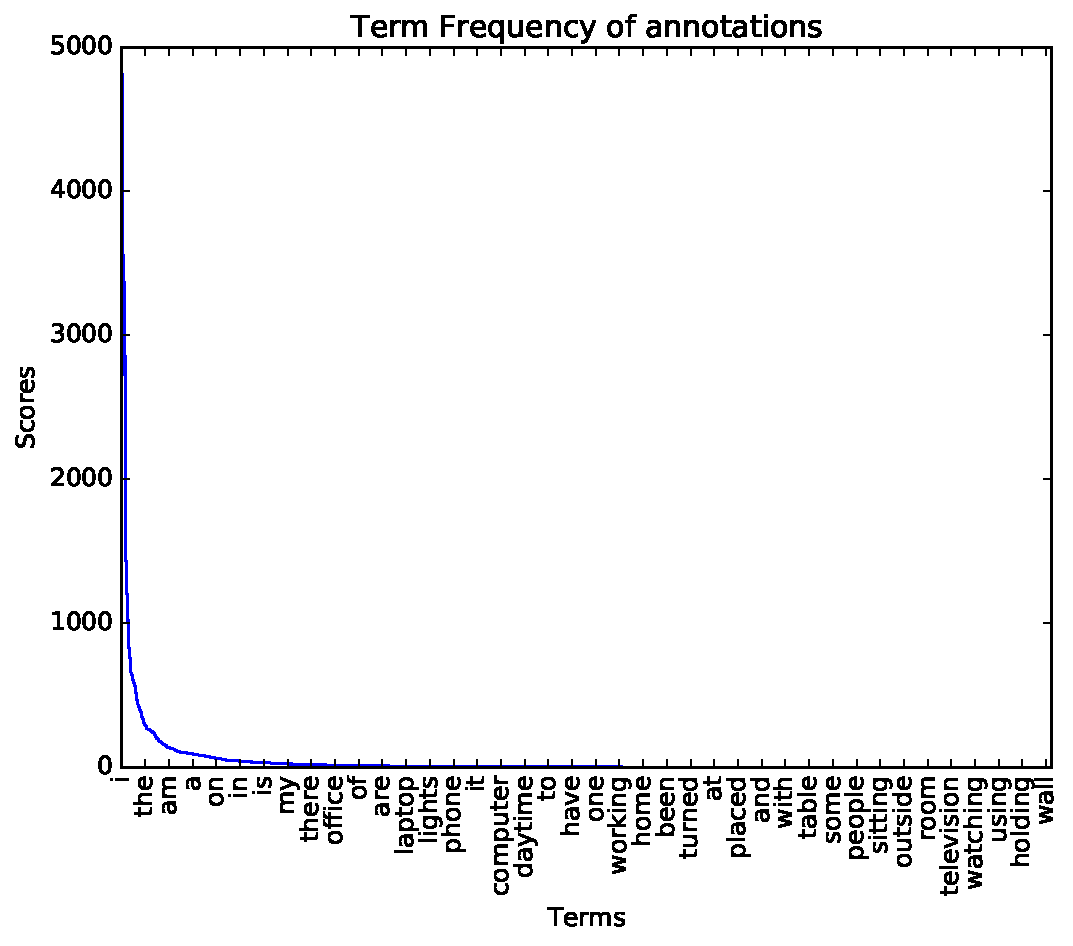
\includegraphics[width=0.7\textwidth]{graphs/tf-scores}
    \caption{Term Frequency scores for concepts in the annotations}
    \label{fig:tf-scores}
\end{figure}

Textual annotations accounted for the highest amount of time taken on average in the collection process. The largest number of annotations collected for a methodology are the query annotations. Qualitative feedback from annotators note that the relevance assessments are the most tedious to collect. Intuitively, formulating a query for a typical search engine does not take a very long time, which can account for the marginal average time for this annotation type. On the other hand, composing (in the annotators mind and physically typing on a keyboard) a descriptive paragraph filled with context and semantics naturally leads to the conclusion that textual annotations do, in fact, take a significant amount of time to annotate. Secondly, the process of completing a relevance assessment involves scrolling and clicking a multitude of times; this time adds up and is evident in the reported average time.

\FloatBarrier
\section{Retrieval Effectiveness}

Results of each experiment are reported as a table which provides the results from \verb|trec_eval| and as a precision-recall graph. The results from only the manually annotated images are displayed first. Table \ref{table:manual-results} presents the \verb|trec_eval| results for the four annotation methodologies \textit{and} the result of combining all four of the methodologies. The  NTCIR-12 LSAT topics are used for experiments. Among other fields, each topic contains a title and a description; these fields are read as input queries. The title field is more representative of what a typical query looks like when issued by a user. The results of running these experiments are visualised as precision-recall graphs in Figures \ref{fig:manual-result-title} and \ref{fig:manual-result-desc}.

The interesting result is the experiments that use the title field as an input: the query annotations perform the best of the four methodologies, however when combining all four collections of annotations together the effectiveness increases slightly, and the precision is higher than the query annotations at high recall. Combining annotations for the experiments that use the description field outperform all four of the methodologies, and the query annotations perform significantly worse.

\begin{table}[ht]
    \begin{tabular}{|c|c|c|c|c|}
        \multicolumn{5}{c}{Topics Titles}\\ \hline
         Methodology & MAP & RR & P@10 & Relevant Retrieved \\ \hline
         Text & 0.3442$^{qc}$ & 0.9223$^{c}$ & 0.8333$^{rc}$ & 1062 \\ \hline
         Tag & 0.5468$^{qcd}$ & 0.9578$^{d}$ & 0.8396$^{rcd}$ & 1040 \\ \hline
         Query & 0.6400$^{tgad}$ & 0.9653$^{rd}$ & 0.8750$^{rd}$ & 1559 \\ \hline
         Relevance Assessment & 0.4815$^{qc}$ & 0.8406$^{qc}$ & 0.6917$^{tgqrd}$ & 831 \\ \hline
         Combined & 0.6495$^{tgrc}$ & 1.000$^{ta}$ & 0.9062$^{tgr}$ & 1612 \\ \hline
         \multicolumn{5}{c}{Topic Descriptions} \\ \hline
         Methodology & MAP & RR & P@10 & Relevant Retrieved \\ \hline
         Text & 0.5285$^{gqc}$ & 0.9792$^{gq}$ & 0.8521$^{gqc}$ & 1088 \\ \hline
         Tag & 0.4627$^{trcd}$ & 0.8928$^{tqcd}$ & 0.7687$^{tqcd}$ & 1055 \\ \hline
         Query & 0.4457$^{tcd}$ & 0.7683$^{tgrcd}$ & 0.5958$^{tgrcd}$ & 1566 \\ \hline
         Relevance Assessment & 0.5219$^{c}$ & 0.9271$^{q}$ & 0.7938$^{tqcd}$ & 972 \\ \hline
         Combined & 0.5855$^{tgqrc}$ & 0.9815$^{gq}$ & 0.8875$^{tgqr}$ & 1613 \\ \hline         
    \end{tabular}
    \caption{MAP, Reciprocal Rank, Precision at 10 scores, and number of relevant retrieved images for the manual annotations. Two tails t-test statistical significance ($p<0.05$) is indicated through the following labels for inter-measurement: text $^t$, tags $^g$, query $^q$, relevance assessment $^r$, combined $^c$. Statistical significance between the same methodology is represented as $^d$.}
    \label{table:manual-results}
\end{table}

\begin{figure}[ht]
    \centering
    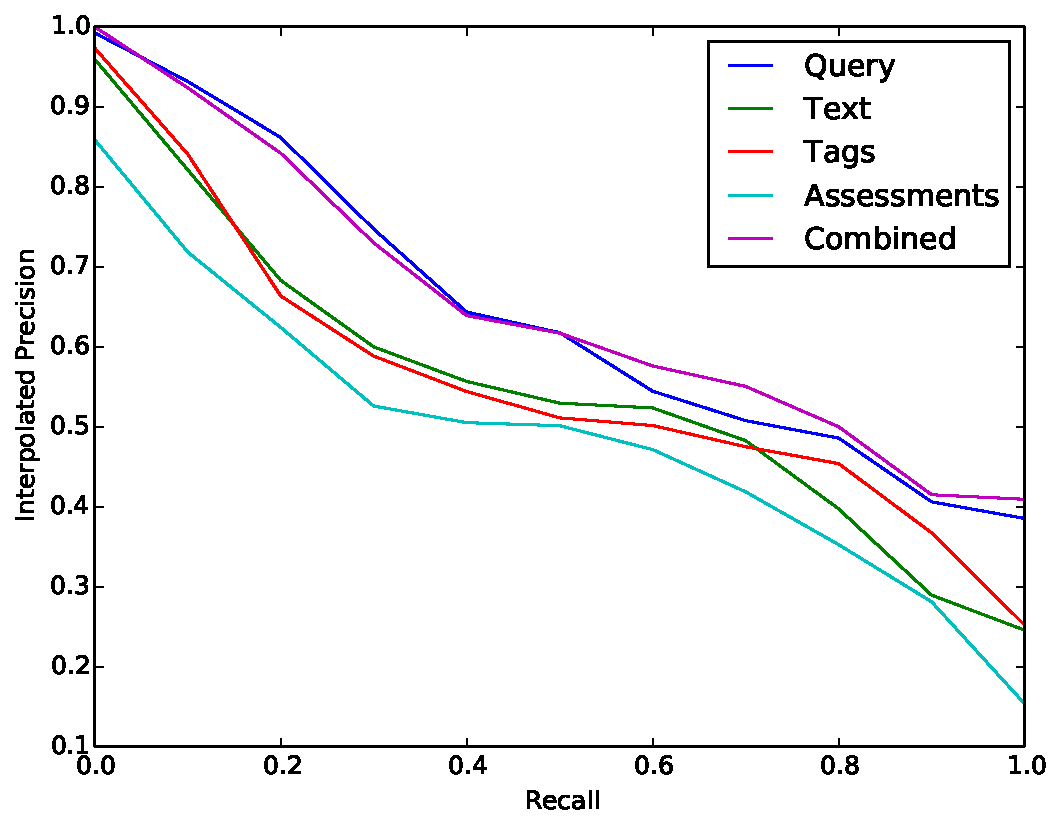
\includegraphics[width=0.8\textwidth]{graphs/manual-title}
    \caption{Precision-recall curves for the manual annotations using topic titles}
    \label{fig:manual-result-title}
\end{figure}

\begin{figure}[ht]
    \centering
    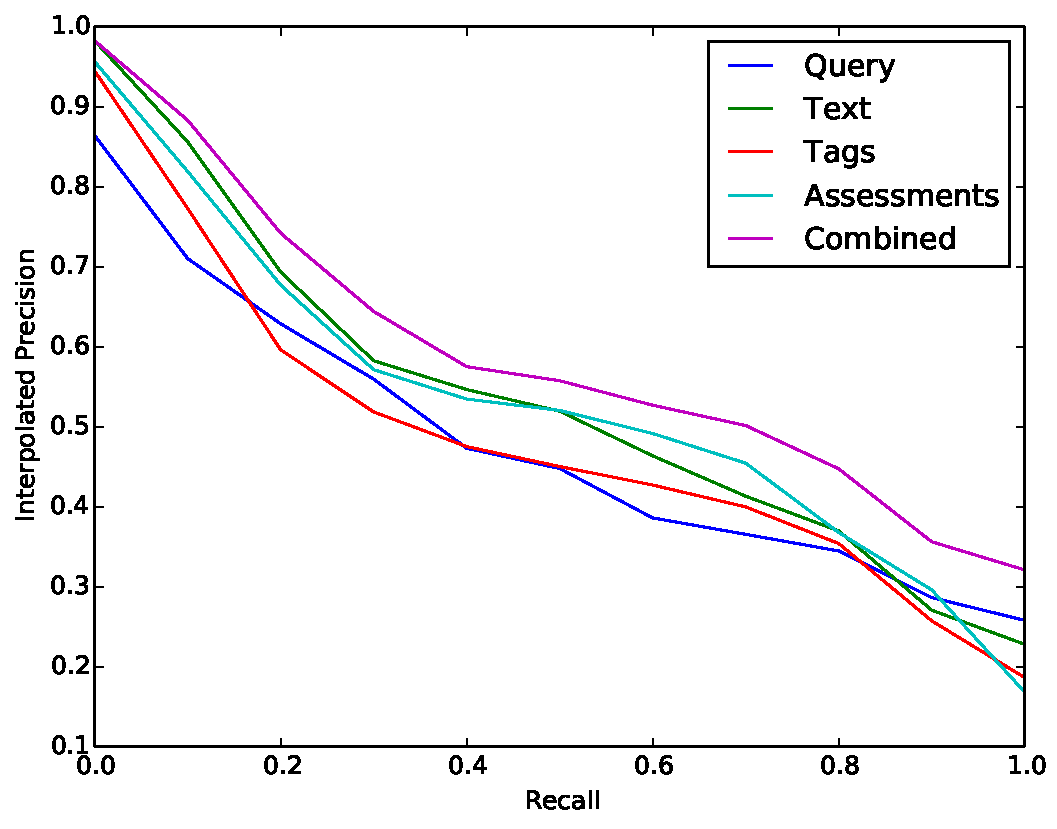
\includegraphics[width=0.8\textwidth]{graphs/manual-desc}
    \caption{Precision-recall curves for the manual annotations using topic descriptions}
    \label{fig:manual-result-desc}
\end{figure}

\FloatBarrier

A neural network framework (neuraltalk2) is trained on the manual textual, tag, and query annotations (i.e. after the manual annotations are collected). Neuraltalk2 is able to produce captions for every image in the collection. The quality of these captions is summarised in Table \ref{table:learnt-results} -- an unfortunate result which could be attributed to the amount of training data. The automatic captions that are generated are evaluated in the same way as the manual annotations. The output of the neural network architecture is formatted to be used in the evaluation pipeline as described in Section \ref{methods:evaluating}. 

There is no clear individual annotation methodology that outperforms the others, the scores are too low to indicate this. Combining the three automatic annotations together does seem to increase the overall precision. The learnt queries do retrieve the most number of images, in a similar result to the manual annotation results.

The number of iterations the neural network architecture covered for each annotation methodology is visualised in Figures \ref{fig:val-loss-1} and \ref{fig:val-loss-2}. The results of the automatic captioning do not get better over time -- in fact they get worse. This is a concerning finding, and it can most likely be attributed the the lack of training examples. The gap between topics with a large number of relevant images and the number of training examples in combination with topics that contain a very low number of relevant images is presumably the contributing factor to the results in these figures.

\begin{table}[ht]
    \centering
    \begin{tabular}{|c|c|c|c|c|}
        \multicolumn{5}{c}{Topic Titles}\\ \hline
         Methodology & MAP & RR & P@10 & Relevant Retrieved\\ \hline
         Text & 0.0048 & 0.0248 & 0.0196 & 187 \\ \hline
         Tag & 0.0083$^{c}$ & 0.0184 & 0.0022 & 136 \\ \hline
         Query & 0.0076 & 0.0174 & 0.0021 & 246 \\ \hline
         Combined & 0.0164$^{g}$ & 0.0393 & 0.0169 & 337 \\ \hline
        \multicolumn{5}{c}{Topic Descriptions}\\ \hline
         Methodology & MAP & RR & P@10 & Relevant Retrieved\\ \hline
         Text & 0.0048 & 0.0232 & 0.0167 & 222 \\ \hline
         Tag & 0.0050 & 0.0184 & 0.0063 & 145 \\ \hline
         Query & 0.0051 & 0.0062 & 0.0062 & 199 \\ \hline
         Combined & 0.0096 & 0.0470 & 0.0187 & 325 \\ \hline
    \end{tabular}
    \caption{MAP, Reciprocal Rank, Precision at 10 scores, and number of relevant retrieved images for the automatically generated annotations. Two tails t-test statistical significance ($p<0.05$) is indicated through the following labels for inter-measurement: text $^t$, tags $^g$, query $^q$, relevance assessment $^r$, combined $^c$. Statistical significance between the same methodology is represented as $^d$.}
    \label{table:learnt-results}
\end{table}

\begin{figure}[ht]
    \centering
    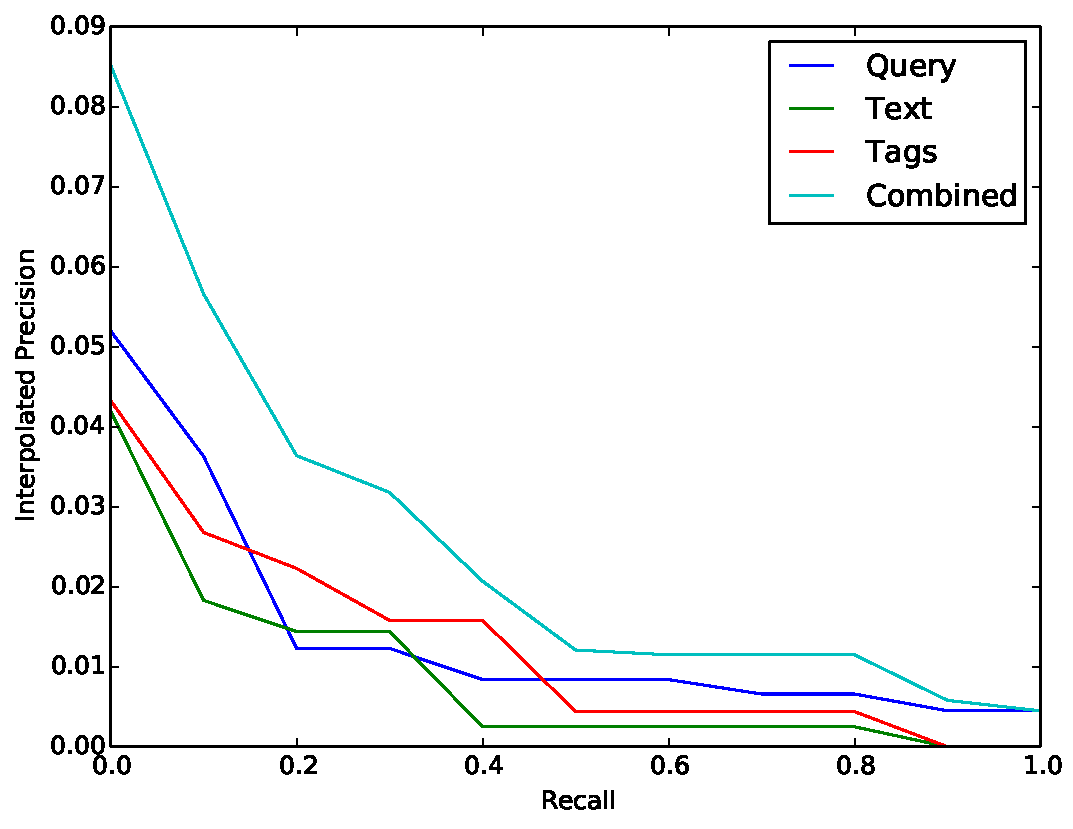
\includegraphics[width=0.8\textwidth]{graphs/auto-title}
    \caption{Precision-recall curves for the learnt annotations using titles}
    \label{fig:manual-result-title}
\end{figure}

\begin{figure}[ht]
    \centering
    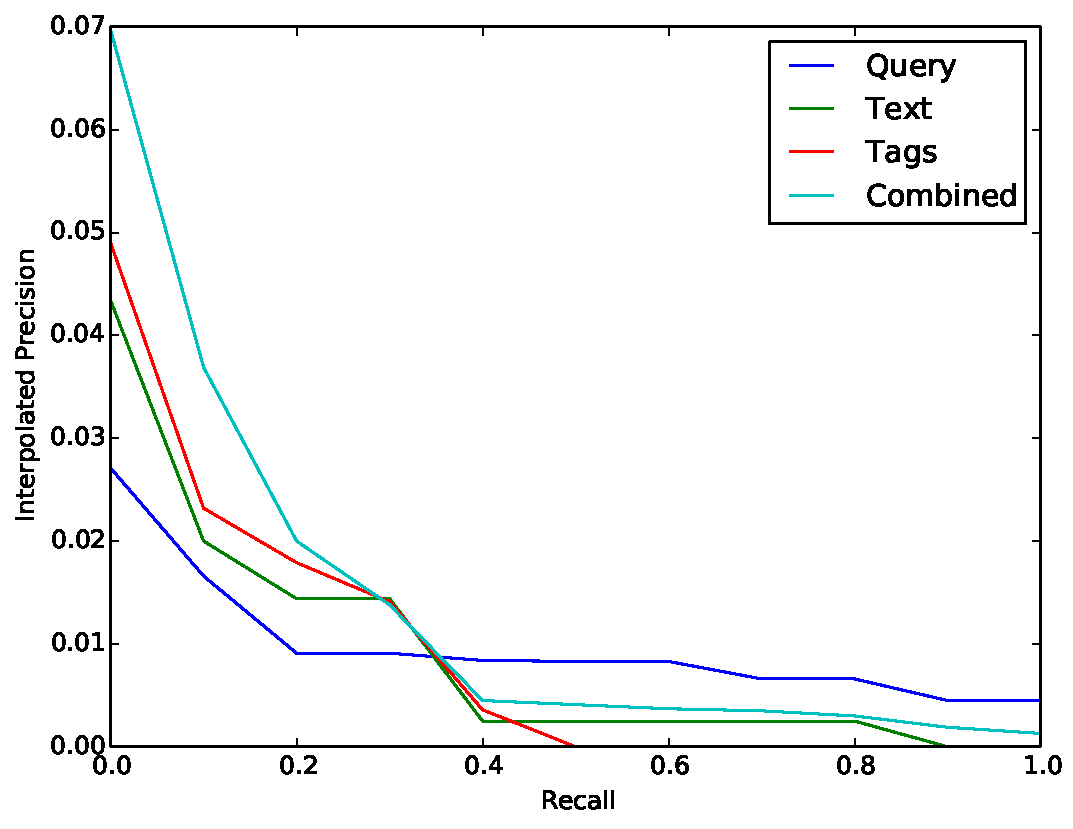
\includegraphics[width=0.8\textwidth]{graphs/auto-desc}
    \caption{Precision-recall curves for the learnt annotations using descriptions}
    \label{fig:manual-result-desc}
\end{figure}

\begin{figure}
    \centering
    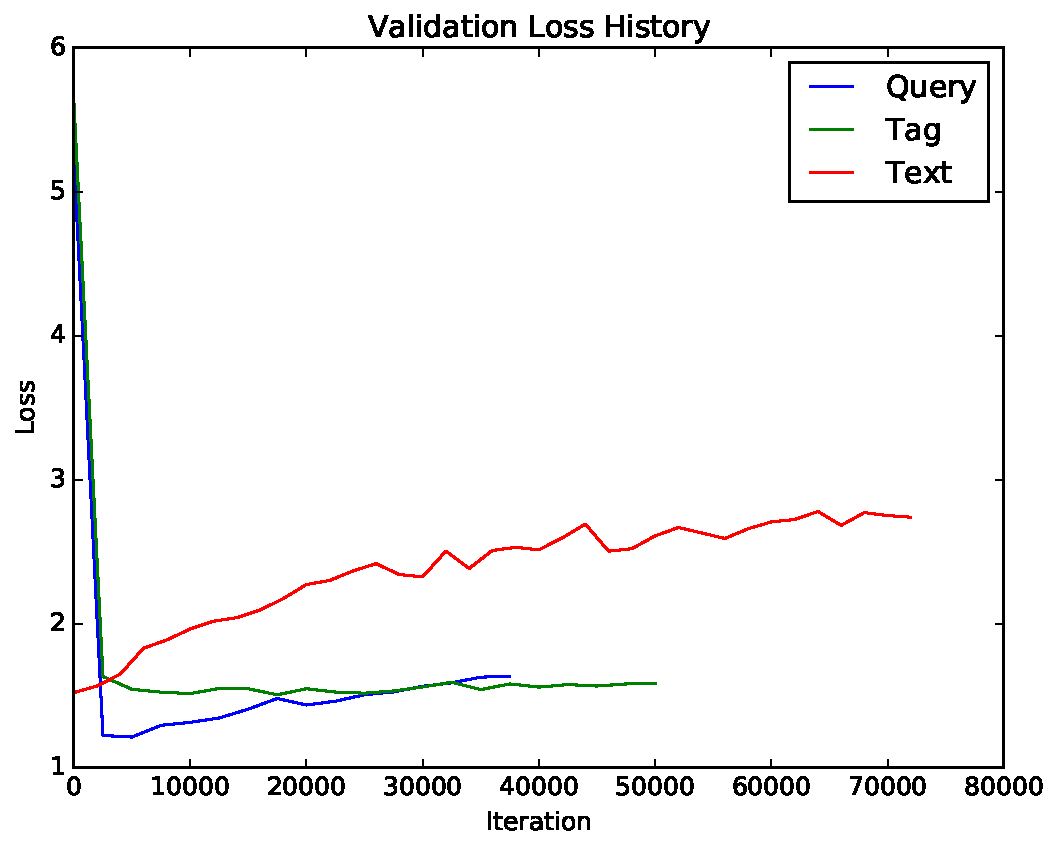
\includegraphics[width=0.7\textwidth]{graphs/initial-validation-loss-history}
    \caption{Validation loss history (\textless 100,000 iterations)}
    \label{fig:val-loss-1}
\end{figure}

\begin{figure}
    \centering
    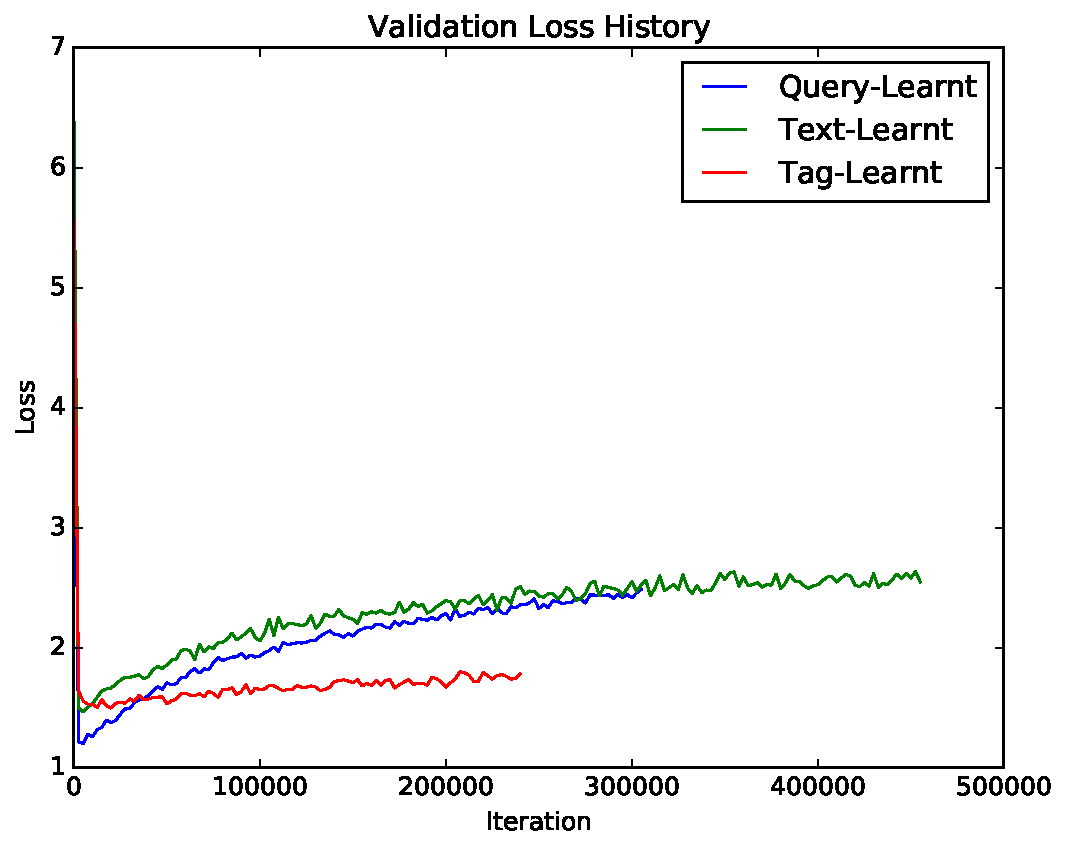
\includegraphics[width=0.7\textwidth]{graphs/validation-loss-history}
    \caption{Validation loss history (\textgreater 200,000 iterations)}
    \label{fig:val-loss-2}
\end{figure}